\documentclass[border=5pt]{standalone}
\usepackage{my_packages}
\usepackage{tikz}
\usetikzlibrary{decorations.markings,decorations.pathreplacing,calc}

\tikzset{help lines/.style={very thin,color=gray!50}} % modify the help lines style
\tikzset{->-/.style={decoration={
  markings,
  mark=at position .5 with {\arrow{>}}},postaction={decorate}}}
  
\begin{document}

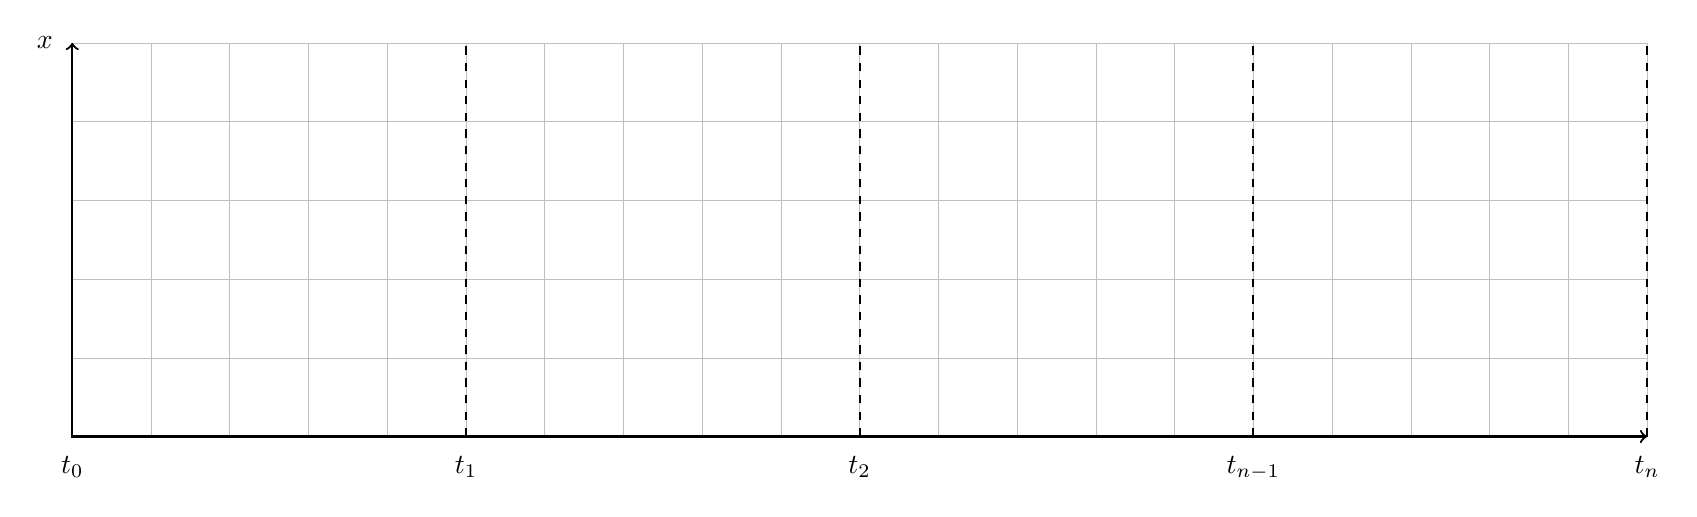
\begin{tikzpicture}[scale=1]
    \draw[help lines] (0,0) grid (20,5) ; %grid

    \node[label=west:\(\vecbf{x}\)] (x0m) at (0,5) {};
    \node[] (x1m) at (5,5) {};
    \node[] (x2m) at (10,5) {};
    \node[] (x3m) at (15,5) {};
    \node[] (xnm) at (20,5) {};

    \node[label=below:\(t_0\)] (t0) at (0,0) {};
    \node[label=below:\(t_1\)] (t1) at (5,0) {};
    \node[label=below:\(t_2\)] (t2) at (10,0) {};
    \node[label=below:\(t_{n-1}\)] (t3) at (15,0) {};
    \node[label=below:\(t_n\)] (tn) at (20,0) {};

    % nodes for each subsegment
    
    % draw axes
    \draw [<->,thick] (tn.center) -- (t0.center) -- (x0m.center);

    % draw segement dividers
    \draw [dashed,thick] (t1.center) -- (x1m.center);
    \draw [dashed,thick] (t2.center) -- (x2m.center);
    \draw [dashed,thick] (t3.center) -- (x3m.center);
    \draw [dashed,thick] (tn.center) -- (xnm.center);


\end{tikzpicture}

\end{document}